%\documentclass[]{openjournal}
\documentclass[iop]{emulateapj}

\bibliographystyle{apj}
\usepackage{graphicx}
\usepackage[suffix=]{epstopdf}
\usepackage[export]{adjustbox}
\usepackage{natbib}
\usepackage{amsmath}
\usepackage{url}
\usepackage{xspace}

%    Make Scientific Notation
\providecommand{\e}[1]{\ensuremath{\times 10^{#1}}}

% make the word Kepler italicized
\newcommand{\Kepler}{\textsl{Kepler}\xspace}


\begin{document}
%%%%%%%%%%%%%%%%%%%%%%
\title{SETI in the Spatial-Temporal Domain: Spatially Coordinated Transits as an ET Signal}

\shorttitle{SETI in the Spatial-Temporal Domain}
\shortauthors{Davenport et al.}

\author{
	James R. A. Davenport\altaffilmark{1,2,3}
	}

\altaffiltext{1}{Corresponding author: James.Davenport@wwu.edu}
\altaffiltext{2}{Department of Physics \& Astronomy, Western Washington University, Bellingham, WA 98225}
\altaffiltext{3}{NSF Astronomy and Astrophysics Postdoctoral Fellow}
 

%%%%%%%%%%%%%%%%%%%%%%%%%%%%%%
\begin{abstract}
Traditional searches for extraterrestrial intelligence (SETI) focuses on temporal or multi-wavelength studies of single stars to detect transient or excess photon emission from artificial sources. However, the latest generation of synoptic time domain surveys enables a spatial-temporal SETI, where signals originate from resolved sources or multiple stars. Here I propose one such SETI approach, which utilizes exoplanet-like transit signals coordinated around multiple stars to indicate the presence of an interstellar civilization. Artificial planets would act as beacons, being placed in orbit around stars surrounding a home star system. The orbital period of each artificial satellite would be proportional to the distance from the beacon star to the home star system. If the orbital period versus beacon distance relationship was known, the exact location of the home system could be determined via triangulation (or trilateration) from a subset of the transit beacons. Current and future exoplanet surveys may be able to detect such spatially coordinated transits around nearby low-mass stars. Importantly, the spatial-temporal domain deserves increased attention from SETI researchers.
\end{abstract}


%%%%%%%%%%%%%%%%%%%%%%%%%%%%%%
\section{Introduction}

In the search for extraterrestrial intelligence (SETI), most approaches focus on direct detection of photons originating from transmission or waste energy. These searches occur over a range of wavelengths, and require extraterrestrials to produce sufficient radiation to be detected apart from their parent star. While this may be feasible at radio wavelengths, it is much more difficult in the optical regime where much of our time domain surveys operate. However,  it is more simple to block significant light from a star than to produce enough to out shine it, which has led to recent studies of time domain data for signatures of transiting artificial structures. 

Previous work has suggested looking for SETI signals from interstellar ``beacons''
\cite{benford2008}
However, most such work has been focused on using lasers or other means to out-shine a parent star, often observed using spectroscopy \cite{reines2002}. This is a very expensive way to stand out, and a slow way to find it, and so far has no success in discovering ET laser emission \cite{tellis2015}


Instead, much cheaper to block light, rather than shine it.
\cite{arnold2005}
on the feasibility of transits for use in SETI detection, and 
\cite{arnold2005a}
on the impact of artificial structures on transits. also this work on that:
\cite{wright2016}.
recent data from \Kepler \citep{borucki2010}, has found weird transit-like signals
\cite{boyajian2015}, 
which some have considered as SETI candidates. However, follow-up observations have yet to yield any confirming signatures, and instead this looks like a YSO w/ comets maybe \citep{lisse2015}.


\cite{arnold2005} note that objects could be placed at interesting spacing along the orbit to encode a pattern or simple message, demonstrating an intelligent origin. However, very little information can be effectively transmitted using eclipses, even with extreme precision in the recovery.


In this work we propose a new type of beacon system, which relies on ET transit signals from multiple stars to collectively ``point'' towards an ET civilization. This system has the advantage of being potentially detectable in the near future via exoplanet searches.




%%%%%%%%%%%%%%%%%%%%%%%%%%%%%%
\section{Coordinated Transits as ET Beacons}



\begin{figure}[]
\centering
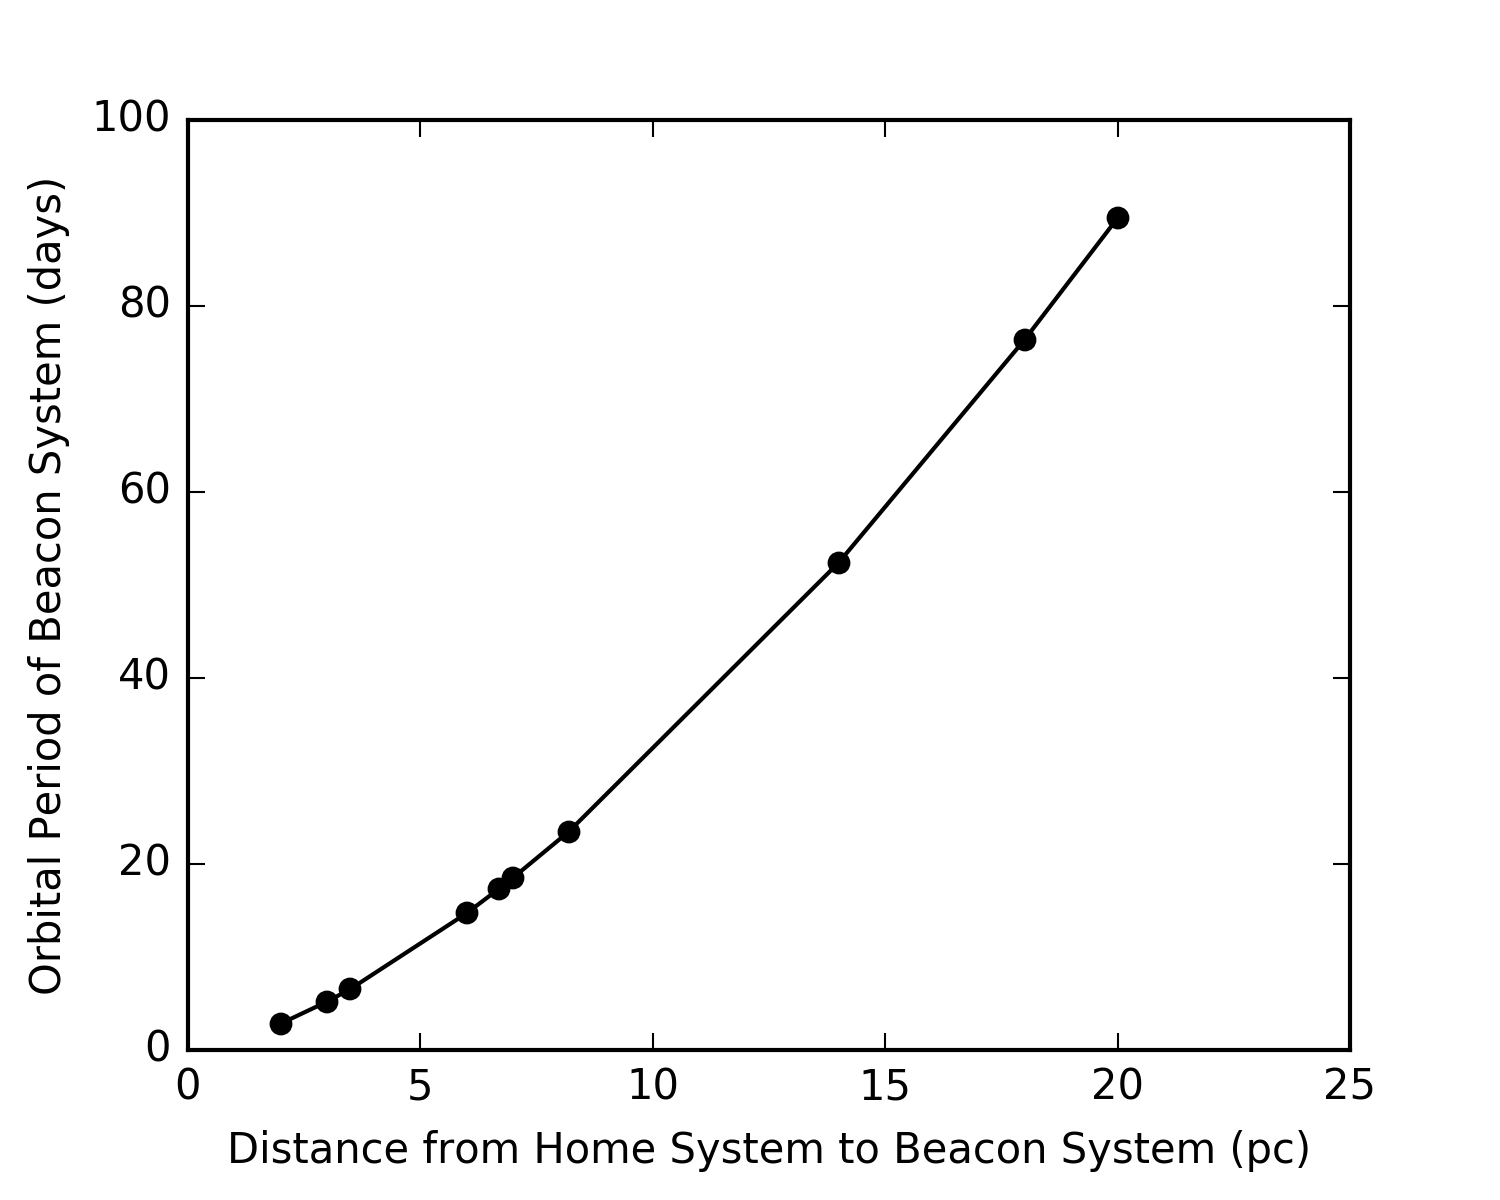
\includegraphics[width=3.5in]{../figures/dist_per.png}
\caption{schematic figure of the signal to detect in 1 dimension}
\label{fig:1d}
\end{figure}


\begin{figure}[]
\centering
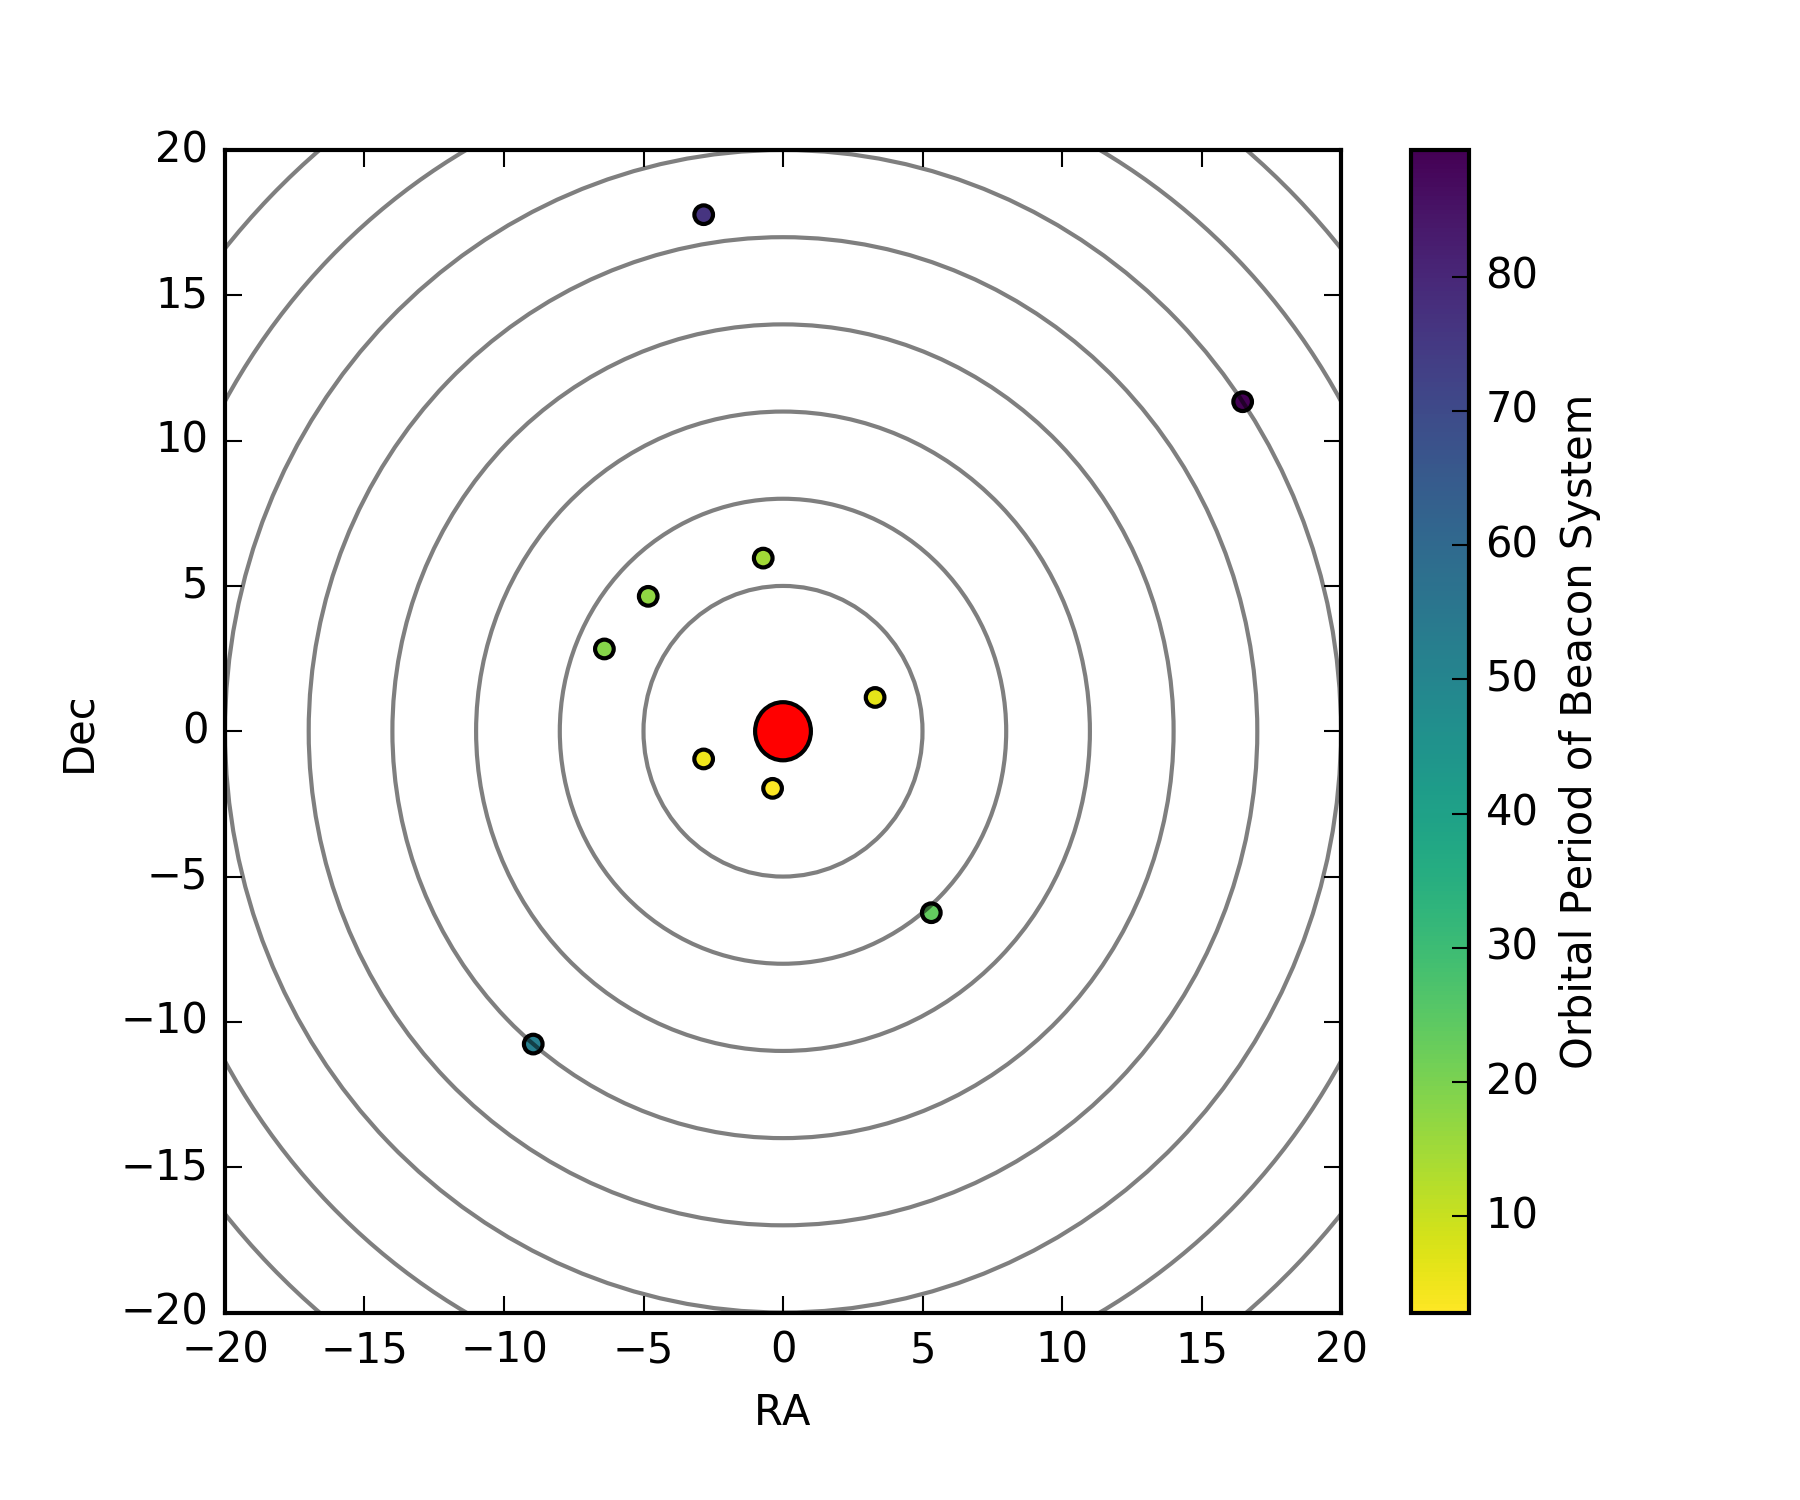
\includegraphics[width=3.5in]{../figures/sky_per.png}
\caption{schematic figure of the signal to detect in 2 dimensions. ra,dec in arbitrary units. red circle in middle is the home system}
\label{fig:2d}
\end{figure}


%%%%%%%%%%%%%%%%%%%%%%%%%%%%%%
\section{Predictions for Upcoming Surveys}
TESS would be great for this in terms of spatial-temporal coverage. 

LSST very good for finding SETI signals of this geometric style, but not ideal for events requiring such dedicating monitoring


%%%%%%%%%%%%%%%%%%%%%%%%%%%%%%
\section{Summary}



%%%%%%%%%%%%%%%%%
\acknowledgments
JRAD is supported by an NSF Astronomy and Astrophysics Postdoctoral Fellowship under award AST-1501418.

\bibliography{/Users/james/research/references}

\end{document}